% Intended LaTeX compiler: pdflatex
\documentclass{scrartcl}
		\usepackage[utf8]{inputenc}
		\usepackage[dvipdfmx]{graphicx}
		\usepackage[dvipdfmx]{color}
		\usepackage[backend=biber,bibencoding=utf8]{biblatex}
		\usepackage{url}
		\usepackage{indentfirst}
		\usepackage[normalem]{ulem}
		\usepackage[dvipdfmx]{hyperref}
		\usepackage{longtable}
		\usepackage{minted}
		\usepackage{fancyvrb}
		\usepackage[top=25truemm,bottom=25truemm,left=25truemm,right=25truemm]{geometry}
		\usepackage[top=25truemm,bottom=25truemm,left=25truemm,right=25truemm]{geometry}
\bibliography{books}
\author{筑波大学情報科学類2年 江畑 拓哉 (201611350)}
\date{}
\title{論理回路実験レポート}
\begin{document}

\maketitle


\section{実験の目的}
\label{sec:org267ad5e}
 バイナリカウンタに、ある条件下である数を引くことのできる回路を作成する。今回での条件とは、4以上の場合を指し、引く数は4である。つまりは4以上の数を持っているカウンタから任意のタイミングで4を引くことのできる回路を作るのである。\\
 たとえば、4から4を引いて0,9から4を引いて5、といった形にしたい。\\

\section{器具及び装置}
\label{sec:org348e921}
 器具及び装置の一覧を以下に示す。\\
\begin{center}
\begin{tabular}{|l|l|l|l|}
\hline
名称 & 個数 & 備考 & 使用理由\\
\hline
●ICトレーナー &  &  & \\
ブレッドボード & 1 &  & 配線のため\\
Vcc(+5V) & 1 & ICトレーナーのブレッドポートに配線 & 電源\\
GND & 1 & ICトレーナーのブレッドポートに配線 & GND\\
7セグメントLED & 1 & 左側を使用 & LED表示のため\\
-左桁用端子(CN4) & 4 & DからAまで使用 & \\
-電源入力端子(CN2) & 1 & 左側のみを接続 & \\
データ出力端子 & 2 & D1,D2を使用 & リセット、演算処理のため\\
データスイッチ & 2 & SW1,SW2を使用(上と対応) & \\
パルス出力端子(DA) & 1 &  & クロックを生むため\\
\hline
●標準ロジックIC &  &  & 回路を作るため\\
74HC00 & 2 & NAND & \\
74HC04 & 1 & NOT & \\
74HC08 & 2 & AND & \\
74HC74 & 2 & D-FF*2を2つ用いた & \\
74HC86 & 1 & XOR & \\
\hline
●その他 &  &  & 配線のため\\
ジャンパ線(ワイヤ) & 大量 & 他の実験者よりもかなり多い(※) & \\
ジャンパ栓(単芯) & 少量 & 他の実験者よりもかなり少ない(※) & \\
\hline
\end{tabular}
\end{center}

※ 他の実験者よりも実装に手間取ったため長いジャンパ線を張り巡らせた。\\

\section{実験経過}
\label{sec:org631d581}

以下に配線図を示す。\\
\begin{figure}[htbp]
\centering
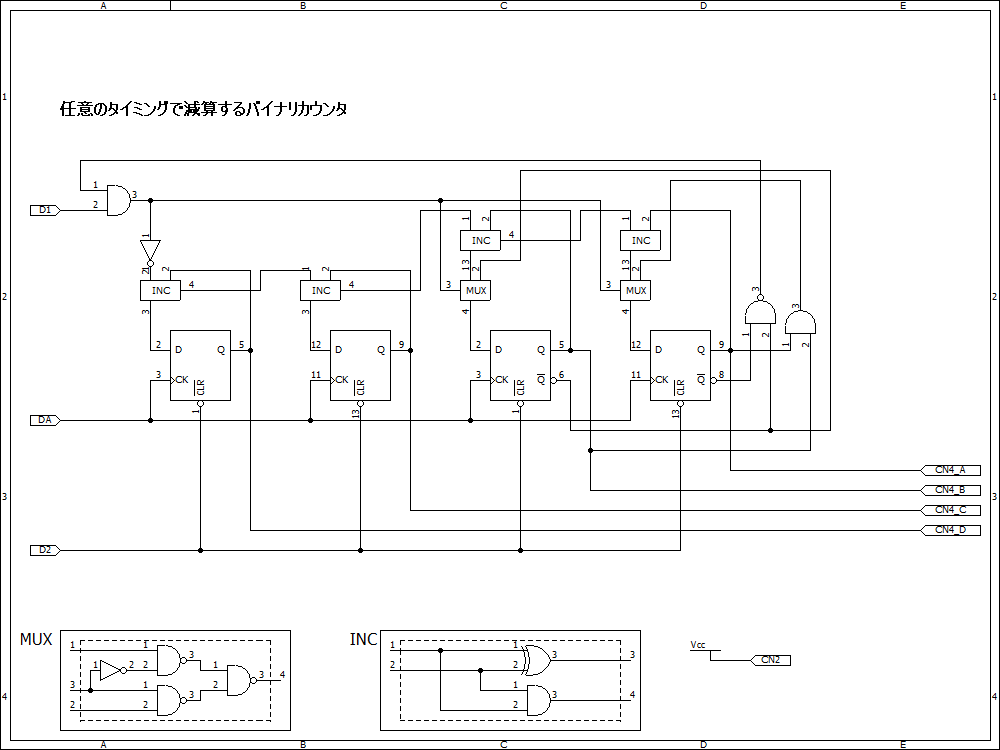
\includegraphics[width=.9\linewidth]{./logicex-2.png}
\caption{\label{fig:org8d59624}
配線図}
\end{figure}
配線を行った後、ICの電源を入れ、クロックを発生させた。\\

\section{実験結果}
\label{sec:orgd80c142}
以下に実行結果を示すためのタイミングチャートを示す。それに続けて説明を加える。\\

\subsection{}
\label{sec:orgf67805d}
\begin{figure}[htbp]
\centering
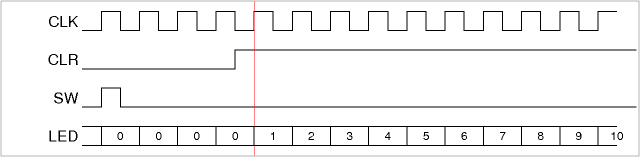
\includegraphics[width=.9\linewidth]{./logic-1.png}
\caption{\label{fig:org68bbc61}
タイミングチャートNo.1}
\end{figure}


 CLR(Active-L)をHにすると、カウントが進み始める。逆にCLRが入っている(Hの)間は0になる。\\

\subsection{}
\label{sec:org2000d9a}
\begin{figure}[htbp]
\centering
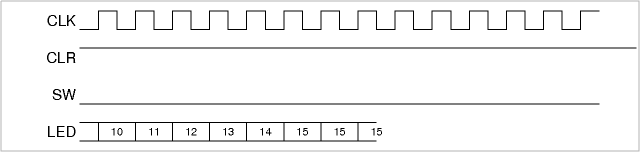
\includegraphics[width=.9\linewidth]{./logic-2.png}
\caption{\label{fig:org9f12d2d}
タイミングチャートNo.2}
\end{figure}


 最終的に16番目の数(15)までカウントが進み、そこで止まる。\\

\subsection{}
\label{sec:org0c836ba}
\begin{figure}[htbp]
\centering
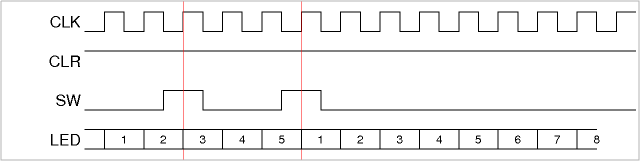
\includegraphics[width=.9\linewidth]{./logic-3.png}
\caption{\label{fig:org707906c}
タイミングチャートNo.3}
\end{figure}

 カウンタが4以上のときスイッチを入れることで4を引かれるが、そうでないとき(今回は2)のときは引き算が行われない。条件が揃っているとき(今回は5)のときは4を引かれる(今回は5 - 4 = 1になる)。尚、引かれるタイミングはクロックが立ち上がったときである。\\

\subsection{}
\label{sec:org695cbbb}
\begin{figure}[htbp]
\centering
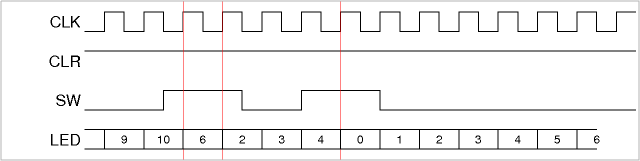
\includegraphics[width=.9\linewidth]{./logic-4.png}
\caption{\label{fig:orgc128aba}
タイミングチャートNo.4}
\end{figure}
 \\

また、4を引いた後にまだ条件を満たしている場合には、更に4を引くことができるので、連続でそれが行われる。更に念のため、4から4を引いて0になるかどうかを確認することができた。\\

\section{考察}
\label{sec:org0578c39}
  今回の課題では4を引く、という文言に踊らされたためにロジックを考える時間を多く取られた。これをもし4を引くのではなく、4( \(=2^2\) )の桁や8 ( \(=2^3\) ) の桁を示すビットを操作する、と読み替えれば問題は途端に容易に解決させることができる。問題の処理についてカルノー図で見てみることにする。(Xはdon't care)\\

\begin{table}[htbp]
\caption{4 = \(2^2\) の桁}
\centering
\begin{tabular}{|l|l|l|}
\hline
4\8 & 0 & 1\\
\hline
0 & X & 1\\
1 & 0 & 0\\
\hline
\end{tabular}
\end{table}

 以上から、4を引く際には、4の桁は元の4の桁の値の反転を取れば良いことがわかった。\\

\begin{table}[htbp]
\caption{4 = \(2^3\) の桁}
\centering
\begin{tabular}{|l|l|l|}
\hline
4\8 & 0 & 1\\
\hline
0 & X & 0\\
1 & 0 & 1\\
\hline
\end{tabular}
\end{table}

 以上から、4を引く際には、8の桁は元の4と8の桁のANDを取れば良いことがわかった。\\

 これによって回路図を作成すれば問題が解けることがわかる。\\
 またこれは次のカウンタの出力なので、これは”半加算器の出力”と選択できるようにすれ良いことがわかる。\\
 \\
 結論として、回路図制作の際には柔軟な試行を持って処理を様々な角度から見直すことが必要なのだということを身にしみて感じた。\\

\section{批判}
\label{sec:org9167088}
   私は、実験内容に関しては十分に噛みごたえのある良い課題内容であって難易度も適切である、と感じているが、周囲の学生を見ると、かなり難航している方もいれば、早々と課題を解決できた方もおり、進捗のばらつきを感じた。\\
   批判に値するかはわからないが、課題の最後になるにつれ難易度が高くなっているため、もう少しTA、教員や友人間で協力できる雰囲気があっても良かったのではないかと考えている。この授業は期末試験がないため、お互いに教え、教えられ合うことでより理解が深まるのではないかと思う。\\
  また、レポートの作成に関して、前回のレポートの採点をもう少し早くするか、例年の、あるいはその年のよくある間違い、減点事項を具体例とともに出していただけると、円滑なレポート提出・採点ができるのではないかと感じている。\\
  \\

\section{参考文献}
\label{sec:org5b5b3b4}
 基本的には自分の頭を用いて作成したが、半加算器などは昨年度必修科目であった論理回路の指定教科書である、「だれにもわかるディジタル回路 \cite{book1}」を用いた。\\


\printbibliography[title=References]\\

\section{発展課題}
\label{sec:org5cf48a0}
以下に発展課題の目的とそれぞれについての内容を記述する。\\

\subsection{実験の目的}
\label{sec:orgc7527da}
 この実験の目的は今までの授業で身につけた知識をより発展的なものにして知識を定着させるためのものだろう。\\
\subsection{課題1:カウンタに任意のリセット回路をつける}
\label{sec:org35adfcf}
10進バイナリカウンタを作成した。\\
\subsubsection{器具及び装置}
\label{sec:org0cf3476}
器具及び装置の一覧を以下に示す。\\
\begin{center}
\begin{tabular}{|l|l|l|l|}
\hline
名称 & 個数 & 備考 & 使用理由\\
\hline
●ICトレーナー &  &  & \\
ブレッドボード & 1 &  & 配線のため\\
Vcc(+5V) & 1 & ICトレーナーのブレッドポートに配線 & 電源\\
GND & 1 & ICトレーナーのブレッドポートに配線 & GND\\
7セグメントLED & 1 & 左側を使用 & LED表示のため\\
-左桁用端子(CN4) & 4 & DからAまで使用 & \\
-電源入力端子(CN2) & 1 & 左側のみを接続 & \\
データ出力端子 & 1 & D2を使用 & リセットのため\\
データスイッチ & 2 & SW2を使用(上と対応) & \\
パルス出力端子(DA) & 1 &  & クロックを生むため\\
\hline
●標準ロジックIC &  &  & 回路を作るため\\
74HC00 & 1 & NAND & \\
74HC08 & 2 & AND & \\
74HC74 & 2 & D-FF*2を2つ用いた & \\
74HC86 & 1 & XOR & \\
\hline
●その他 &  &  & 配線のため\\
ジャンパ線(ワイヤ) & 大量 & 他の実験者よりもかなり多い & \\
ジャンパ栓(単芯) & 少量 & 他の実験者よりもかなり少ない & \\
\hline
\end{tabular}
\end{center}

\subsubsection{実験経過}
\label{sec:org951f4c3}
以下に配線図を示す。\\
\begin{figure}[htbp]
\centering
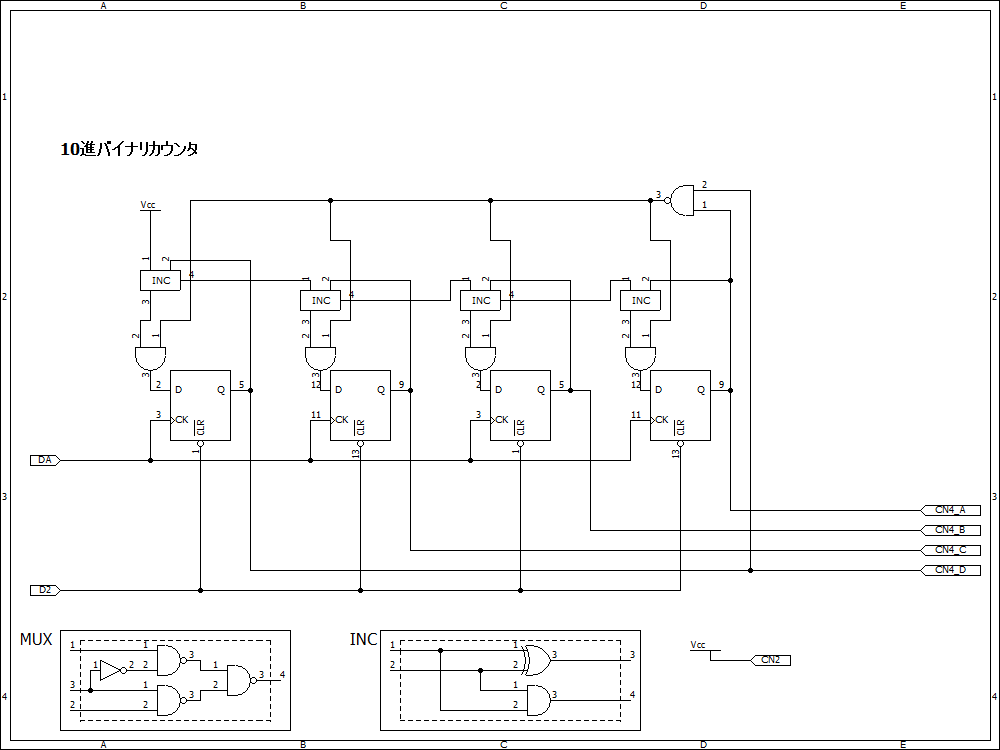
\includegraphics[width=.9\linewidth]{./logice-1.png}
\caption{\label{fig:org16b6468}
配線図}
\end{figure}
配線を行った後、ICの電源を入れ、クロックを発生させた。\\

\subsubsection{実験結果}
\label{sec:org22eb5f4}
以下のように動作し、これが10進カウンタとしての役割を満たしていることを確認した。\\
\begin{figure}[htbp]
\centering
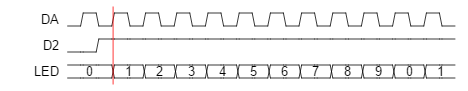
\includegraphics[width=.9\linewidth]{./logictime-1.png}
\caption{\label{fig:org8a22957}
タイミングチャートNo.1}
\end{figure}

\subsubsection{考察}
\label{sec:orgdd68073}
 作り方としては、9( = 8 + 1)であることを検出したならばこれをキーに次の出力を0にするのである。今回はこの機能をANDを用いることで作成した。\\
 実験結果を見る限り問題なく動作していることは明らかである。\\
 考察として挙げるものは特にはないが、カウントアップを行っているうちに途中停止の機能を追加したいとも思った。実際1を足していた部分をVccからD9などに接続してカウントを停止できるような機能を実験外で追加した。\\

\subsubsection{}
\label{sec:orgc5e59b1}
\subsubsection{批判}
\label{sec:org5312a2e}
この課題では批判は何もなかった。\\

\subsection{課題2:特定の条件で 1 サイクルのみパルスを発生する}
\label{sec:org46843f7}
 特定の条件で一サイクルのみパルスを発生させた。今回その特定の条件とは、2つの入力がどちらもHになったときのことを指す。\\
\subsubsection{器具及び装置}
\label{sec:org93b94f5}
器具及び装置の一覧を以下に示す。\\
\begin{center}
\begin{tabular}{|l|l|l|l|}
\hline
名称 & 個数 & 備考 & 使用理由\\
\hline
●ICトレーナー &  &  & \\
ブレッドボード & 1 &  & 配線のため\\
Vcc(+5V) & 1 & ICトレーナーのブレッドポートに配線 & 電源\\
GND & 1 & ICトレーナーのブレッドポートに配線 & GND\\
データ出力端子 & 1 & D0/D1を使用 & 入力\\
データスイッチ & 2 & SW0/SW1を使用(上と対応) & \\
パルス出力端子(DA) & 1 &  & クロックを生むため\\
データ入力スイッチ & 1 & I0を使用 & 出力\\
\hline
●標準ロジックIC &  &  & 回路を作るため\\
74HC08 & 1 & ANDを2つ用いた & \\
74HC74 & 1 & D-FFを2つ用いた & \\
\hline
●その他 &  &  & 配線のため\\
ジャンパ線(ワイヤ) & 少々 &  & \\
\hline
\end{tabular}
\end{center}
\subsubsection{実験経過}
\label{sec:org5b44647}
 以下に配線図を示す。\\
\begin{figure}[htbp]
\centering
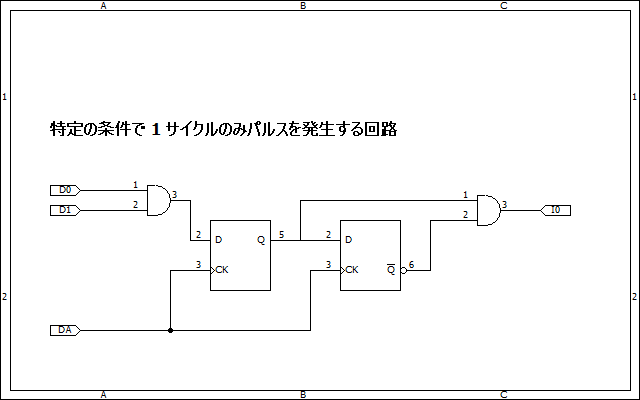
\includegraphics[width=.9\linewidth]{./logice-2.png}
\caption{\label{fig:orgfc1a476}
配線図}
\end{figure}
配線を行った後、ICの電源を入れ、入力を変化させた行った。\\
\subsubsection{実験結果}
\label{sec:org5568dfd}
以下に動作のタイミングチャートを示す\\
\begin{figure}[htbp]
\centering
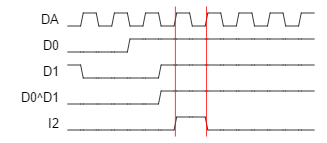
\includegraphics[width=.9\linewidth]{./logictime-2.png}
\caption{\label{fig:org9cfaf73}
タイミングチャートNo.2}
\end{figure}

\subsubsection{考察}
\label{sec:org0e6d889}
 資料に示された同期微分回路とほぼ変わらない設計となっている。\\
 実験結果から正しい動作を行うことが明らかである。特に異常な動作を示さなかった。\\
\subsubsection{批判}
\label{sec:org1da2ecb}
 1サイクルの意味を解釈することが難しかったため、1クロック分と書き換えた方が良いと考えている。\\
\subsection{課題3:リセット後一回のみ動作する回路}
\label{sec:orga456987}
 リセットを押された後に一回だけ動作する回路を作った。\\
\subsubsection{器具及び装置}
\label{sec:orga175da5}
器具及び装置の一覧を以下に示す。\\
\begin{center}
\begin{tabular}{|l|l|l|l|}
\hline
名称 & 個数 & 備考 & 使用理由\\
\hline
●ICトレーナー &  &  & \\
ブレッドボード & 1 &  & 配線のため\\
Vcc(+5V) & 1 & ICトレーナーのブレッドポートに配線 & 電源\\
GND & 1 & ICトレーナーのブレッドポートに配線 & GND\\
データ出力端子 & 1 & D0を使用 & 入力\\
データスイッチ & 2 & SW0を使用(上と対応) & \\
クロック出力端子(DA) & 1 &  & クロックを生むため\\
パルス入力スイッチ & 1 & I0を使用 & 出力\\
\hline
●標準ロジックIC &  &  & 回路を作るため\\
74HC00 & 1 & NANDを1つ用いた & \\
74HC04 & 1 & NOTを1つ用いた & \\
74HC74 & 1 & D-FFを1つ用いた & \\
\hline
●その他 &  &  & 配線のため\\
ジャンパ線(ワイヤ) & 少々 &  & \\
\hline
\end{tabular}
\end{center}
\subsubsection{実験経過}
\label{sec:orgc742a7e}
 以下に配線図を示す。\\
\begin{figure}[htbp]
\centering
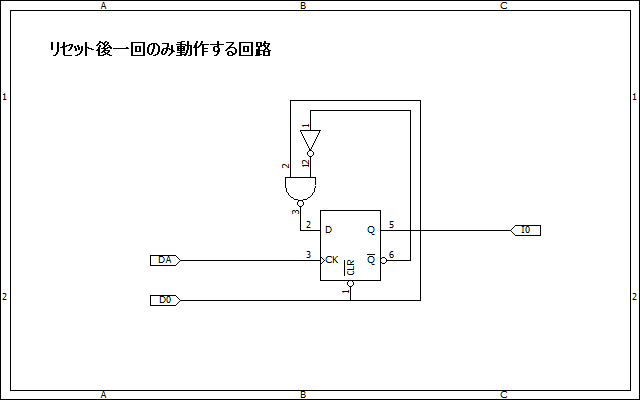
\includegraphics[width=.9\linewidth]{./logice-3.png}
\caption{\label{fig:org52439b6}
配線図}
\end{figure}
配線を行った後、ICの電源を入れ、入力を変化させた行った。\\
\subsubsection{実験結果}
\label{sec:org7bb37c5}
以下に動作のタイミングチャートを示す\\
\begin{figure}[htbp]
\centering
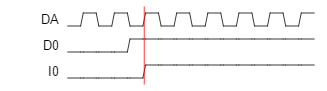
\includegraphics[width=.9\linewidth]{./logictime-3.png}
\caption{\label{fig:org7ce3630}
タイミングチャートNo.3}
\end{figure}
\subsubsection{考察}
\label{sec:orga688ef5}
 出力を次の入力に入れることで解決した。\\
 クリアをして、その入力を受けて次のクロックで出力がH担っているを事が確認できた。入力をクリアから別のものに分けたものが次の課題の重要な位置要素になっている。\\
\subsubsection{批判}
\label{sec:org9bfae88}
この課題では批判は何もなかった。\\

\subsection{課題4:ボタンを押した時一回のみ作動する回路}
\label{sec:orgea9e2d5}
ボタンが押されたら、そこからカウントアップする8進タイマーを作成した。\\
\subsubsection{器具及び装置}
\label{sec:orgd22d2cc}
器具及び装置の一覧を以下に示す。\\
\begin{center}
\begin{tabular}{|l|l|l|l|}
\hline
名称 & 個数 & 備考 & 使用理由\\
\hline
●ICトレーナー &  &  & \\
ブレッドボード & 1 &  & 配線のため\\
Vcc(+5V) & 1 & ICトレーナーのブレッドポートに配線 & 電源\\
GND & 1 & ICトレーナーのブレッドポートに配線 & GND\\
7セグメントLED & 1 & 左側を使用 & LED表示のため\\
-左桁用端子(CN4) & 4 & DからAまで使用 & \\
-電源入力端子(CN2) & 1 & 左側のみを接続 & \\
データ出力端子 & 2 & D0を使用 & リセットのため\\
データスイッチ & 2 & SW0を使用(上と対応) & \\
データ入力スイッチ & 1 & I0を使用 & ボタンが押されたことを検出\\
パルス出力端子(DA) & 1 &  & カウントの開始のため\\
クロック出力端子(CK) &  &  & クロックを生むため\\
\hline
●標準ロジックIC &  &  & 回路を作るため\\
74HC00 & 1 & NANDを1つ用いた & \\
74HC04 & 1 & NOTを1つ用いた & \\
74HC08 & 1 & ANDを3つ用いた & \\
74HC74 & 2 & D-FF*2を2つ用いた & \\
74HC86 & 1 & XORを3つ用いた & \\
\hline
●その他 &  &  & 配線のため\\
ジャンパ線(ワイヤ) & 大量 &  & \\
ジャンパ栓(単芯) & 少量 &  & \\
\hline
\end{tabular}
\end{center}
\subsubsection{実験経過}
\label{sec:orgc3575ed}
 以下に配線図を示す。\\
\begin{figure}[htbp]
\centering
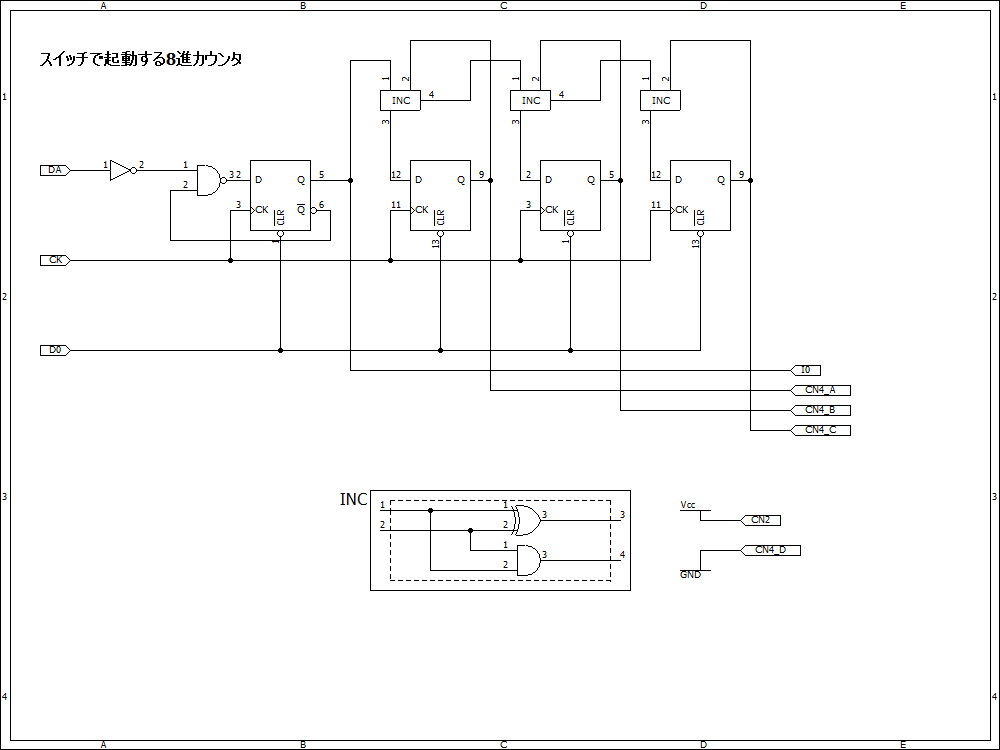
\includegraphics[width=.9\linewidth]{./logice-4.png}
\caption{\label{fig:orge37c5e3}
配線図}
\end{figure}
配線を行った後、ICの電源を入れ、入力を変化させた行った。\\
\subsubsection{実験結果}
\label{sec:org3b14328}
以下に動作のタイミングチャートを示す\\
\begin{figure}[htbp]
\centering
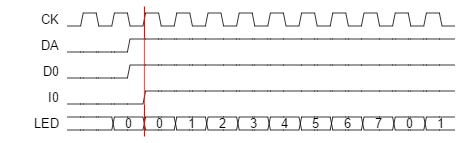
\includegraphics[width=.9\linewidth]{./logictime-4.png}
\caption{\label{fig:orgf0186d6}
タイミングチャートNo.3}
\end{figure}
\subsubsection{考察}
\label{sec:org29d19f3}
 課題3で行ったことをバイナリカウンタに追加することで機能を満たす回路を作成した。\\
 期待通りの動作が行われたことがわかったが、はじめに動作を起こすか確認するための1クロックがどうしても気になってしまった。D-FFのクロックを複数持てないため仕方のないことだが、分集をするなどの対策を施したいと思った。\\
 また、ボタンを押したときその動作を記憶する、という動作を行うためにはボタンを押した動作が1クロック分は継続していることが望ましい、という問題も残った。今回はクロックを分集できるだけのICがなかったため、あるいは複数のクロックを発生することができなかったため、こちらも実装はできなかった。\\
\subsubsection{批判}
\label{sec:org8030815}
この課題では批判は何もなかった。\\

\subsection{参考文献}
\label{sec:org18d6af8}
 9章のものと同じものを用いた。\\
\end{document}
